\documentclass[crop,tikz]{standalone}

\begin{document}
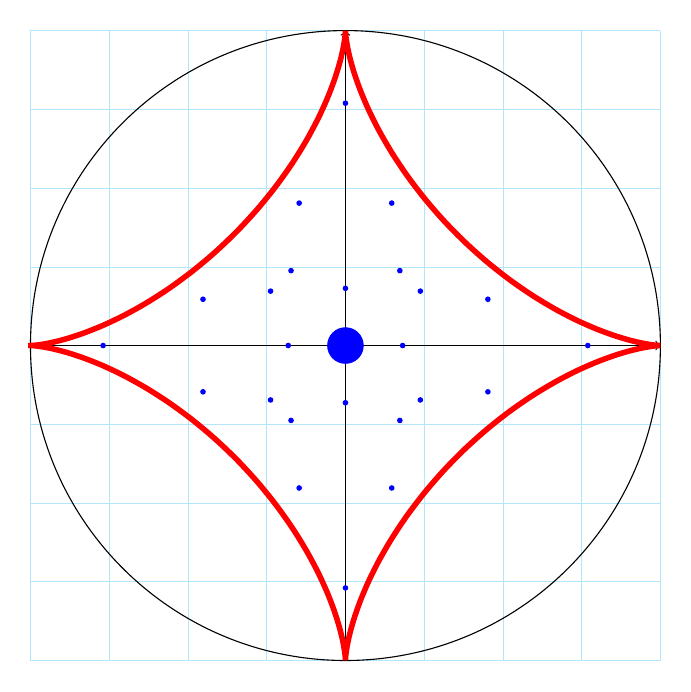
\begin{tikzpicture}
\def\a{1} \def\b{4} \def\scale{1}
\draw[cyan!30,very thin] ({-\b*\scale},{-\b*\scale}) grid ({\b*\scale},{\b*\scale});
\draw[->] ({-\b*\scale},0) -- ({\b*\scale},0);
\draw[->] (0,{-\b*\scale}) -- (0,{\b*\scale});
\draw (0,0) circle ({\b*\scale});
\draw[line width=2pt,red] plot[samples=100,domain=0:\a*360,smooth,variable=\t] ({\scale*((\b-\a)*cos(\t)+\a*cos((\b-\a)*\t/\a)},{\scale*((\b-\a)*sin(\t)-\a*sin((\b-\a)*\t/\a)});

\draw[blue,fill=blue] (0.7265425280053608,-0.0) circle (4*0.200000000000000pt);
\draw[blue,fill=blue] (-0.5877852522924731,-1.8090169943749475) circle (4*0.200000000000000pt);
\draw[blue,fill=blue] (0.0,0.0) circle (4*1.60000000000000pt);
\draw[blue,fill=blue] (0.0,0.7265425280053608) circle (4*0.200000000000000pt);
\draw[blue,fill=blue] (0.9510565162951533,0.6909830056250525) circle (4*0.200000000000000pt);
\draw[blue,fill=blue] (0.6909830056250525,0.9510565162951535) circle (4*0.200000000000000pt);
\draw[blue,fill=blue] (-3.077683537175253,0.0) circle (4*0.200000000000000pt);
\draw[blue,fill=blue] (0.9510565162951535,-0.6909830056250525) circle (4*0.200000000000000pt);
\draw[blue,fill=blue] (-0.6909830056250525,-0.9510565162951535) circle (4*0.200000000000000pt);
\draw[blue,fill=blue] (-1.8090169943749475,-0.5877852522924731) circle (4*0.200000000000000pt);
\draw[blue,fill=blue] (-1.8090169943749475,0.5877852522924731) circle (4*0.200000000000000pt);
\draw[blue,fill=blue] (1.8090169943749475,-0.5877852522924731) circle (4*0.200000000000000pt);
\draw[blue,fill=blue] (0.5877852522924731,1.8090169943749475) circle (4*0.200000000000000pt);
\draw[blue,fill=blue] (-0.6909830056250525,0.9510565162951535) circle (4*0.200000000000000pt);
\draw[blue,fill=blue] (0.5877852522924729,-1.8090169943749475) circle (4*0.200000000000000pt);
\draw[blue,fill=blue] (-0.5877852522924729,1.8090169943749475) circle (4*0.200000000000000pt);
\draw[blue,fill=blue] (0.6909830056250525,-0.9510565162951535) circle (4*0.200000000000000pt);
\draw[blue,fill=blue] (-0.7265425280053608,0.0) circle (4*0.200000000000000pt);
\draw[blue,fill=blue] (-0.9510565162951533,-0.6909830056250525) circle (4*0.200000000000000pt);
\draw[blue,fill=blue] (0.0,-3.077683537175253) circle (4*0.200000000000000pt);
\draw[blue,fill=blue] (-0.9510565162951535,0.6909830056250525) circle (4*0.200000000000000pt);
\draw[blue,fill=blue] (1.8090169943749475,0.5877852522924731) circle (4*0.200000000000000pt);
\draw[blue,fill=blue] (0.0,3.077683537175253) circle (4*0.200000000000000pt);
\draw[blue,fill=blue] (3.077683537175253,0.0) circle (4*0.200000000000000pt);
\draw[blue,fill=blue] (-0.0,-0.7265425280053608) circle (4*0.200000000000000pt);
\end{tikzpicture}

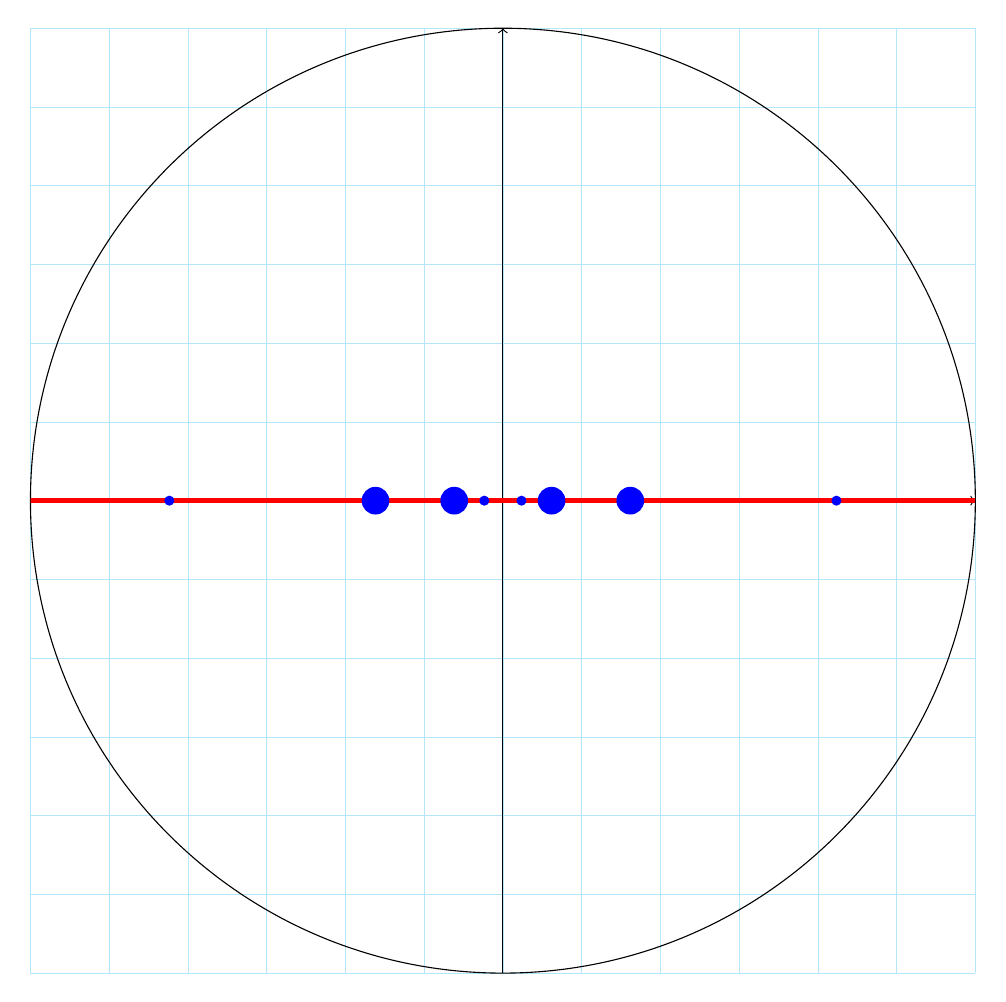
\begin{tikzpicture}
\def\a{1} \def\b{2} \def\scale{3}
\draw[cyan!30,very thin] ({-\b*\scale},{-\b*\scale}) grid ({\b*\scale},{\b*\scale});
\draw[->] ({-\b*\scale},0) -- ({\b*\scale},0);
\draw[->] (0,{-\b*\scale}) -- (0,{\b*\scale});
\draw (0,0) circle ({\b*\scale});
\draw[line width=2pt,red] plot[samples=100,domain=0:\a*360,smooth,variable=\t] ({\scale*((\b-\a)*cos(\t)+\a*cos((\b-\a)*\t/\a)},{\scale*((\b-\a)*sin(\t)-\a*sin((\b-\a)*\t/\a)});

\draw[blue,fill=blue] (-0.2360679774997898,0.0) circle (4*0.400000000000000pt);
\draw[blue,fill=blue] (-1.618033988749895,0.0) circle (4*1.20000000000000pt);
\draw[blue,fill=blue] (-0.6180339887498949,0.0) circle (4*1.20000000000000pt);
\draw[blue,fill=blue] (0.6180339887498949,0.0) circle (4*1.20000000000000pt);
\draw[blue,fill=blue] (1.618033988749895,0.0) circle (4*1.20000000000000pt);
\draw[blue,fill=blue] (0.2360679774997898,0.0) circle (4*0.400000000000000pt);
\draw[blue,fill=blue] (4.23606797749979,0.0) circle (4*0.400000000000000pt);
\draw[blue,fill=blue] (-4.23606797749979,0.0) circle (4*0.400000000000000pt);
\end{tikzpicture}

\end{document}